
Due to some physical limitations in the realization of quantum hardware, today's quantum computers are qualified as noisy intermediate-scale quantum (NISQ) hardware. NISQ hardware is characterized by a few of qubits (50 to a few hundred) and noisy operations. Moreover, current realizations of superconducting quantum chips do not have the ideal all-to-all connectivity between qubits, but rather at most a nearest-neighbor connectivity. Due to these constraints, most quantum algorithms cannot be able to directly executed on the NISQ devices. Dynamically remapping logical qubits to physical qubits is needed to enable the two-qubit gates in the algorithm. This is called the qubit mapping problem.

The qubit mapping problem has been proved to be NP-Complete~\cite{siraichi2018qubit}. Considering the time-complexity, \MindQuantum\ chooses a swap-based bidirectional heuristic algorithm, named SABRE~\cite{li2019tackling}.

Fig.~\ref{fig:qubit-mapping-sample} gives a sample of qubit mapping.
The physical hardware has its own physical connected graph. When we map the logical qubits to physical qubits, some two-qubit gates may not be able to realize, because two qubits are not connected in the physical connected graph. The trivial solution is using the swap gate. By some swap-operations, the logical circuit can be realized.

\begin{figure}
	\centering
	\begin{subfigure}{0.1\textwidth}
		\centering
		\includegraphics[width=\textwidth]{8.2_figures/example_topo}
		\caption{Physical topology graph.}
	\end{subfigure}
	\begin{subfigure}{0.3\textwidth}
		\centering
		\includegraphics[width=0.9\textwidth]{8.2_figures/example_original}
		\caption{Logical circuit.}
	\end{subfigure}

	\begin{subfigure}{0.45\textwidth}
		\centering
		\includegraphics[width=\textwidth]{8.2_figures/example_updated}
		\caption{Fixed circuit.}
	\end{subfigure}

	\caption{An example of qubit mapping.}
	\label{fig:qubit-mapping-sample}
\end{figure}

The goal of the algorithm is to reduce the number of swap gates and the circuit depth.

Firstly, we can generate a directed acyclic graph (DAG) to represent the constraints between the two-qubit gates in the given quantum circuit. Single qubit gates can always be executed, therefore there is no need to consider them. We can label every two-qubit gate as $g_i(q_j, q_k)$, which means $g_i$ acts on $q_j$ and $q_k$. If $g_x(q_i, q_j)$ is followed by $g_y(q_j, q_k)$, then we add an edge $(g_x, g_y)$ to the DAG. Fig.~\ref{fig:qubit-mapping-dag} shows an example of DAG generation.

\begin{figure}
	\centering
	\begin{subfigure}{0.49\textwidth}
		\centering
		\includegraphics[width=\textwidth]{8.2_figures/dag_circuit}
		\caption{Quantum circuit.}
	\end{subfigure}
	\begin{subfigure}{0.49\textwidth}
		\centering
		\includegraphics[width=\textwidth]{8.2_figures/dag_dag}
		\caption{Generated DAG.}
	\end{subfigure}
	\caption{An example of DAG generation.}
	\label{fig:qubit-mapping-dag}
\end{figure}

The core idea of the algorithm is trivial. Similar to topological sorting, we can construct a front layer which need to be executed now. If a gate can be executed under the current mapping, execute it and update the front layer. When there is no gate that can be executed, calculate available SWAPs. At last, we choose the SWAP which has the minimal heuristic function value.

The basic heuristic function is from the nearest neighbor cost function. For two physical qubit $Q_i$ and $Q_j$, $D[Q_i][Q_j]$ stands for the nearest distance in the physical connected graph. For a given front layer $F$ and current mapping $\pi$, the basic function is defined as
Eq.~\eqref{eq:qubit-mapping-h-basic}.
\begin{equation} \label{eq:qubit-mapping-h-basic}
	H_{\text{basic}} = \sum_{g \in F} D[\pi (g.q_1)][\pi (g.q_2)].
\end{equation}

$H_{\text{basic}}$ only considers the front layer. If we want to look ahead, we can add an extended set $E$, which contains some closet successors of the gates from $F$. The size of $E$ is flexible, depending on how much look-ahead ability we want. Also, the gates in $F$ should have a higher priority than $E$. So a weight parameter $0 \leq W < 1$ is added.

Up to now, the heuristic function tends to reduce the number of SWAP gates. We also want to reduce the depth of the circuit. There is a trade-off between them. We add a parameter $decay$ to each qubit. If a qubit already has many operations on it, it will have a bigger $decay$. Using $decay$, the algorithm will tend to choose those qubits that have fewer operations and increase the parallelism of the circuit. The fixed heuristic function is given by
Eq.~\eqref{eq:qubit-mapping-h}.
\begin{equation} \label{eq:qubit-mapping-h}
	\begin{aligned}
		H =    & \max \left( decay(SWAP.q_1), decay(SWAP.q_2) \right)                \\
		\times & \Big\lbrace \frac{1}{|F|} \sum_{g \in F} D[\pi(g.q_1)][\pi(g.q_2)]  \\
		+      & \frac{W}{|E|} \sum_{g \in E} D[\pi(g.q_1)][\pi(g.q_2)] \Big\rbrace.
	\end{aligned}
\end{equation}

Lastly, there is a problem of the initial mapping. It has been proved that initial mapping could have a huge impact on the final result. Here we use a method introduced in \cite{li2019tackling}.
Fig.~\ref{fig:qubit-mapping-initial-mapping}
shows the procedure of updating the initial mapping.

\begin{figure}
	\centering
	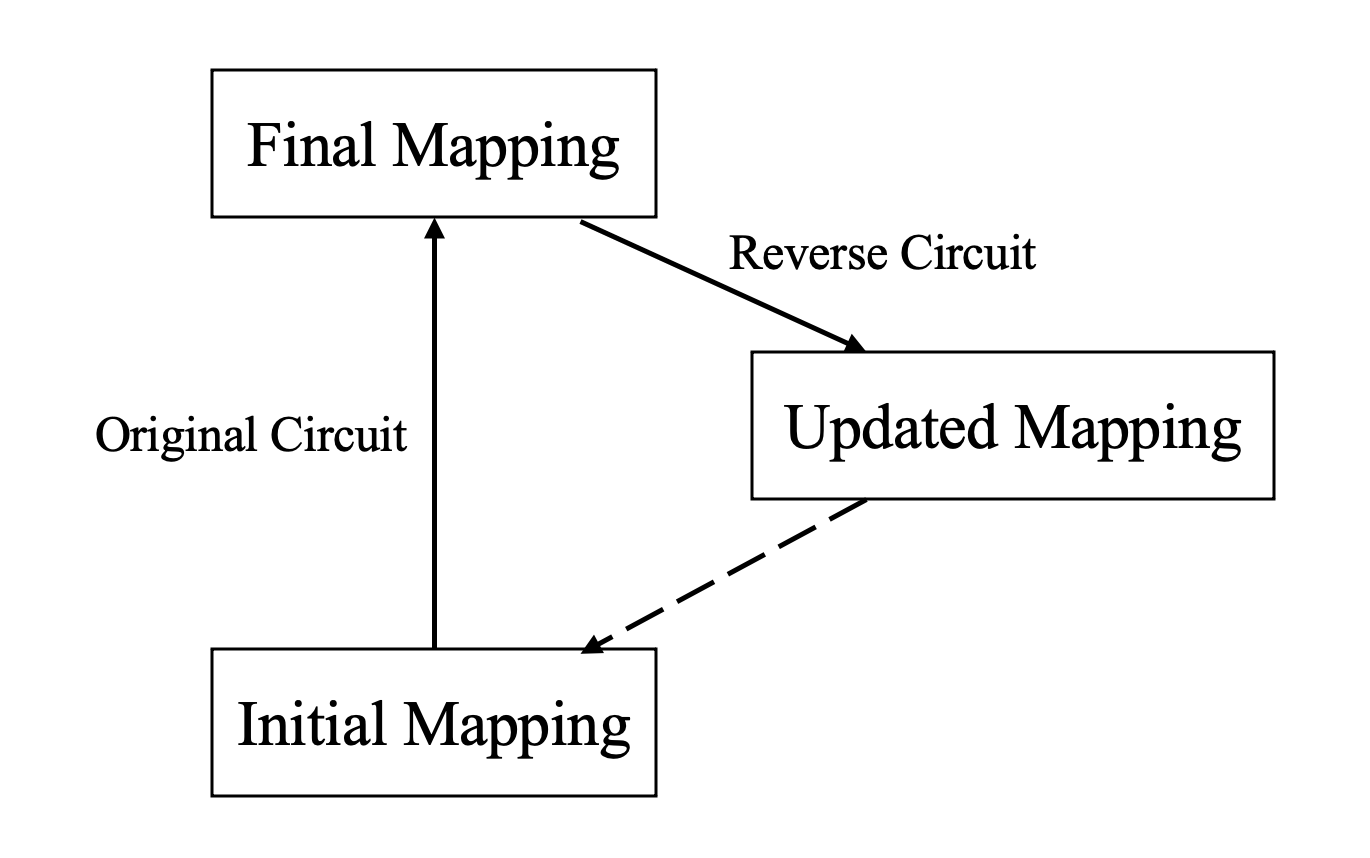
\includegraphics[width=0.45\textwidth]{8.2_figures/initial_mapping.png}
	\caption{Initial mapping update procedure.}
	\label{fig:qubit-mapping-initial-mapping}
\end{figure}

Here we introduce how to use SABRE in \MindQuantum. We can use \code{QubitNode} and \code{QubitsTopology} to generate physical topology graph.

\begin{lstlisting}
from mindquantum.device import QubitNode, QubitsTopology
from mindquantum.io.display import draw_topology

n: int = 5
topology = QubitsTopology([QubitNode(i, poi_x=i) for i in range(n)])
draw_topology(topology)
\end{lstlisting}

The above code defines a topology graph which contains 5 nodes. \code{QubitNode(i, poi_x=i)} defines a \code{QubitNode} whose ID is \code{i} and x-axis coordinate is \code{i}. \code{draw_topology} is used to draw the SVG Fig.~\ref{fig:qubit-mapping-topo1}.

\begin{figure}
	\centering
	\begin{subfigure}{0.2\textwidth}
		\centering
		\includegraphics[width=0.8\textwidth]{8.2_figures/topo_1}
		\caption{Disconnected graph.}
		\label{fig:qubit-mapping-topo1}
	\end{subfigure}
	\begin{subfigure}{0.2\textwidth}
		\centering
		\includegraphics[width=0.8\textwidth]{8.2_figures/topo_2}
		\caption{Connected graph.}
		\label{fig:qubit-mapping-topo2}
	\end{subfigure}
	\caption{Define a topology graph which contains 5 nodes.}
\end{figure}

We can also use \code{q1 >> q2} or \code{q1 << q2} to connect different nodes, and use \code{q1 > q2} or \code{q1 < q2} to disconnect nodes. The following code connects Fig.~\ref{fig:qubit-mapping-topo1} and generate Fig.~\ref{fig:qubit-mapping-topo2}.

\begin{lstlisting}
for i in range(n-1):
topology[i] << topology[i+1]
draw_topology(topology)
\end{lstlisting}

\MindQuantum\ also defines some useful structures. The following code defines a linear topology in Fig.~\ref{fig:qubit-mapping-linear} and a grid topology in Fig.~\ref{fig:qubit-mapping-grid1}.

\begin{lstlisting}
from mindquantum.device import LinearQubits, GridQubits

t1 = LinearQubits(3)
t2 = GridQubits(3,4)
draw_topology(t1)
draw_topology(t2)
\end{lstlisting}

We can also modify existing graph. The following codes remove a node, isolate a node, change a node's color, change a node's position and add a new edge. Fig.~\ref{fig:qubit-mapping-grid2} shows the modified graph.

\begin{figure}[H]
	\centering

	\begin{subfigure}{0.1\textwidth}
		\includegraphics[width=0.9\textwidth]{8.2_figures/linear}
		\caption{Linear.}
		\label{fig:qubit-mapping-linear}
	\end{subfigure}
	\begin{subfigure}{0.15\textwidth}
		\includegraphics[width=0.9\textwidth]{8.2_figures/grid1}
		\caption{Grid.}
		\label{fig:qubit-mapping-grid1}
	\end{subfigure}
	\begin{subfigure}{0.2\textwidth}
		\includegraphics[width=0.9\textwidth]{8.2_figures/grid2}
		\caption{Modified.}
		\label{fig:qubit-mapping-grid2}
	\end{subfigure}

	\caption{Some useful structures and modified graph.}
\end{figure}

\begin{lstlisting}
t2.remove_qubit_node(0)
t2.isolate_with_near(5)
t2.set_color(6, "#ff0000")
t2.set_position(3, 4, 0)
t2[3] << t2[11]
draw_topology(t2)
\end{lstlisting}

Combined with a given topology graph, we can use SABRE algorithm to generate a qubit mapping for any logical quantum circuit. The following codes define a topology graph \code{topo} and a logical circuit \code{circ}. SABRE solver needs 4 parameters:
\begin{itemize}
	\item \code{iter_num}: Number of iterations to generate initial mapping.
	\item \code{w}: $W$ parameter in Eq.~\eqref{eq:qubit-mapping-h}.
	\item \code{delta1}: Decay of single gates.
	\item \code{delta2}: Decay of CNOT gate.
\end{itemize}
The solver returns three parts:
\begin{itemize}
	\item \code{new_circ}: Physical circuit.
	\item \code{initial_mapping}: A list that represents the initial mapping. Here lower-case q stands for logical qubits and capital Q stands for physical qubits. For example, \code{[3, 2, 0, 1]} means logical $q_0$ stores in physical $Q_3$, $q_1$ in $Q_2$, $q_2$ in $Q_0$ and $q_3$ in $Q_1$.
	\item \code{final_mapping}: A list that represents the final mapping.
\end{itemize}
Fig.~\ref{fig:qubit-mapping-physical-circuit} shows a possible solution.

\begin{lstlisting}
topo = GridQubits(2, 2)
display_svg(draw_topology(topo))

from mindquantum.core.circuit import Circuit
from mindquantum.algorithm.mapping import SABRE

circ = Circuit().h(0).h(1).h(2).x(1, 0).x(2, 1).x(0, 2)
print("Logical circuit:")
display_svg(circ.svg())

solver = SABRE(circ, topo)
new_circ, init_mapping, final_mapping = solver.solve(5, 0.5, 0.3, 0.2)
print("Physical circuit:")
print(f"initial mapping: {init_mapping}")
print(f"  final mapping: {final_mapping}")
display_svg(new_circ.svg())
\end{lstlisting}

\begin{figure}
	\centering
	\begin{subfigure}{0.1\textwidth}
		\includegraphics[width=0.8\textwidth]{8.2_figures/topo_3}
		\caption{Physical topology graph.}
		\label{fig:qubit-mapping-physical-topo}
	\end{subfigure}
	\begin{subfigure}{0.35\textwidth}
		\includegraphics[width=\textwidth]{8.2_figures/logical}
		\caption{Logical circuit.}
		\label{fig:qubit-mapping-logical-circuit}
	\end{subfigure}
	\begin{subfigure}{0.45\textwidth}
		\includegraphics[width=0.9\textwidth]{8.2_figures/physical}
		\caption{A possible physical circuit. The initial mapping is \code{[3, 2, 0, 1]} and final mapping is \code{[1, 2, 0, 3]}.}
		\label{fig:qubit-mapping-physical-circuit}
	\end{subfigure}

	\caption{An example of SABRE algorithm.}
\end{figure}

There are also some shortcomings. Current \MindQuantum\ only supports connected topology graphs. If physical topology is not connected, users have to allocate logical qubits to physical connected subgraphs manually.
Another one is gates' type. Current version only supports single gates and CNOT gate. Any quantum circuit can be realized by single gates and CNOT, therefore it's not a big problem.

% Test \code{hello world} .
% - Eq.~\eqref{}
% - Fig.~\ref{}
% - \code{}
